\documentclass[paper=a4, fontsize=11pt]{scrartcl}

%\usepackage[T1]{fontenc} 
\usepackage[english]{babel} 
\usepackage{amsmath}
\usepackage{amsfonts}
\usepackage{amsthm}
\usepackage{amssymb}
\usepackage{changepage}
\usepackage{titlesec}
\usepackage{tikz}
\usepackage{subcaption}
\usetikzlibrary{positioning}
\usepackage{sectsty} 
\sectionfont{\centering \normalfont \scshape}
\subsectionfont{\normalfont}
\subsubsectionfont{\normalfont}

\usepackage{fancyhdr} 
\pagestyle{fancyplain} 
\fancyhead{} 
\fancyfoot[L]{} 
\fancyfoot[R]{} 
\fancyfoot[C]{\thepage} 
\renewcommand{\headrulewidth}{0pt} 
\renewcommand{\footrulewidth}{0pt} 
\setlength{\headheight}{13.6pt} 

\usepackage{enumitem}
\newcommand{\subscript}[2]{$#1 _ #2$}
\newcommand{\Zn}[1]{\mathbb{Z}_{#1}}
\newcommand{\cyc}[1]{\left< #1 \right>}
\newcommand{\nextline}{$ $ \newline \vspace{-0.15in}}
\newcommand{\horrule}[1]{\rule{\linewidth}{#1}} 
\newcommand{\ball}[2]{$B({#1};{#2})$}
\newcommand{\overbar}[1]{
	\mkern 1.5mu \overline{\mkern-1.5mu\raisebox{0pt}[\dimexpr\height+0.5mm\relax]{$#1$}\mkern-1.5mu}\mkern 1.5mu
}

\title{	
	\normalfont \normalsize 
	\textsc{Konkuk University Dept. Of Physics} \\ [25pt] %Konkuk University Dept. of Physics
	\horrule{1pt} \\[0.4cm] 
	\huge Group Theory \\
	\vspace{0.1in}
	\Large 2019 Spring Semester
	\horrule{1pt} \\[0.4cm] 
}

\author{Youngwan Kim} 
\date{\normalsize\today} 

\newtheorem{theorem}{Thm}
\newtheorem{definition}{Def}
%\newtheorem{examples}{Examples}
\newtheorem{example}{Ex}
\newtheorem{lemma}{Lem}
\newtheorem*{remark}{Remark}
\newtheorem*{recall}{Recall}

\begin{document}
	
\maketitle	

\section{Binary Operations}
\vspace{0.25in}

\begin{definition}
	For a set $S$, a map $\ast : S \to S$ is a \textbf{binary operation}. \\
\end{definition}

\begin{example}
$ $ \newline
\vspace{-0.15in}
\begin{enumerate}
	\item f \\
\end{enumerate}
\end{example}

\begin{definition}
	For a given set $S$, and a binary operation $\ast : S \to S$,
	\begin{enumerate}
		\item $\ast$ is \textbf{commutative} if for every $a,b \in S$, $a \ast b = b \ast a$
		\item $\ast$ is \textbf{associative} if for every $a,b,c \in S$, $(a \ast b) \ast c = a \ast ( b\ast c)$ \\
	\end{enumerate}
\end{definition}

\begin{remark}
	For associative binary operators, we can write $(a \ast b) \ast c = a \ast ( b\ast c)$ as just $a \ast b \ast c$. \\
\end{remark}

\begin{definition}
	Let $\ast$ be a binary operation on $S$. Also let $H$ be a subset of $S$. If $H$ is closed under $\ast$, we say that $\ast : H \times H \to H$ is the \textbf{induced operation} of $\ast$ on $H$.\\
\end{definition}


\section{Isomorphic Binary Structures}
\vspace{0.25in}

\begin{definition}
	Let $\ast$ be a binary operation on $S$. Then $(S,\ast)$ is called a \textbf{binary algebraic structure}.\\
\end{definition}

\begin{definition}
	Let $(S,\ast),(S',\ast')$ be binary algebraic structures. An \textbf{isomorphism} is a map $f:S\to S'$ with the following conditions :\\
	\begin{enumerate}
		\item $f$ is a bijection.
		\item $f(a\ast b)=f(a)\ast' f(b)$ for all $a,b \in S$.\\
	\end{enumerate}
	If such isomorphism exists between such binary structures, we say that $S$ is \textbf{isomorphic} to $S'$ and denote it as $S\simeq S'$. \\
\end{definition}

\begin{remark}
	For maps between binary algebraic structures such that only the second condition of \textbf{Def 5} holds, are called \textbf{homomorphisms}.\\
\end{remark}

\begin{example}
	list of isomorphic structures \\
\end{example}

\begin{lemma}
	Suppose $(S,\ast) \simeq (S',\ast')$. If $S$ is commutative, then $(S',\ast')$ is also commutative.\\
\end{lemma}

\begin{proof}
	Let $\phi:S\to S'$ be the isomorphism. For any $a',b' \in S'$ we can let $a' = \phi(a)$ and $b'=\phi(b)$ for some $a,b \in S$ as $\phi$ is a bijection. As $S$ is commutative, $a\ast b = b \ast a$ which implies that $\phi(a \ast b) = \phi(b \ast a)$. Then as $\phi$ is an isomorphism, $\phi(a \ast b)=\phi(a) \ast' \phi(b)=a'\ast'b'$ and also for the other term, $\phi(b \ast a)=\phi(b) \ast' \phi(a)=b'\ast'a'$. Thus for every $a',b' \in S'$, as $a'\ast'b'=b'\ast'a$, $(S',\ast')$ is also commutative.\\
\end{proof}

\begin{definition}
	Let $(S,\ast)$ be a binary structure. An element $e \in S$ is an identity element if for every $a \in S$, $a \ast e = e \ast a = a$.\\
\end{definition}

\begin{example}
	Examples of some binary structures and their identity elements.\\
\end{example}

\begin{theorem}
	Suppose $e$ is an identity element of $(S,\ast)$ and consider an isomorphism $\phi:S\to S'$. Then $\phi(e)$ is also an identity element in $(S',\ast')$.\\
\end{theorem}

\begin{proof}
	For any $a' \in S'$, since $\phi$ is bijective, there exists some $a \in S$ such that $\phi(a)=a'$. We will show that $a' \ast' \phi(e) =  \phi(e) \ast' a' = a'$. The left hand side shows up to be, \\
	\begin{equation}\nonumber
		a' \ast' \phi(e) = \phi(a) \ast' \phi(e)= \phi(a \ast e) = \phi(a) = a'
	\end{equation}\\
	and the right hand side shows up to be, \\
	\begin{equation}\nonumber
		 \phi(e) \ast' a' =  \phi(e) \ast' \phi(a) = \phi(e \ast a) = \phi(a) = a'
	\end{equation}\\
	Thus as this holds for every element in $S'$, we can say that $\phi(e)$ is an identity element in $S'$.\\
\end{proof}

\begin{theorem}
	The identity element of any binary algebraic structure is unique.\\
\end{theorem}

\begin{proof}
	Consider two identity elements $e,e'$ for a certain binary algebraic structure. As both ar e identities, \\
	\begin{equation} \nonumber
		e \ast e' = e' \ast e = e
	\end{equation}\\
	and also 
	\begin{equation} \nonumber
		e' \ast e = e \ast e' = e'
	\end{equation} \\
	which implies that $e=e'$ for any other identity elements if there exists, and thus we can conlude that the identity element uniquely exists.\\
\end{proof}

\vspace{0.25in}
\section{Groups}
\vspace{0.25in}

\begin{definition}
	A binary algebraic structure $(G,\ast)$ is a \textbf{group} if the following conditions holds
	\begin{enumerate}[label=(\subscript{G}{{\arabic*}})]
		\item \textbf{Associativity} : $\forall a,b,c \in G : (a \ast b) \ast c = a \ast (b \ast c)$
		\item \textbf{Identity element} : $\exists e \in G : \forall a \in G , e \ast a = a \ast e = a$
		\item \textbf{Inverse element} : $\exists b \in G : \forall a \in G , b \ast a = a \ast b = e$\\
	\end{enumerate}
\end{definition}

\begin{example}
	content...\\
\end{example}

\begin{definition}
	Let $(G,\ast)$ be a group. $G$ is \textbf{abelian} if $\ast$ is commutative.\\
\end{definition}

\begin{lemma}
	Let $G$ be a group and $x \in G$. Then $x$ has a unique inverse element.\\
\end{lemma}

\begin{proof}
	Suppose $y,z$ are both the inverse element of $x$. Which is equivalent to,\\
	\begin{equation}\nonumber
		\begin{split}
		 &\iff x \ast y =e , x\ast z =e \implies x\ast y = x \ast z \\
		 &\implies y \ast(x\ast y) = y \ast(x \ast z) \\ 
		 &\implies  (y \ast x)\ast y = (y \ast x) \ast z \\
		 &\implies e \ast y = e \ast z \\
		 &\implies y = z \\
		\end{split}
	\end{equation}
\end{proof}

\begin{theorem}
	Let $G$ be a group where $a,b,c \in G$. Then the following holds 
	\begin{enumerate}
		\item \textbf{left cancellation} : $a \ast b = a \ast c \implies b =c$
		\item \textbf{right cancellation} : $b \ast a = c \ast a \implies b = c$ \\
	\end{enumerate}
\end{theorem}

\begin{theorem}
	Let $G$ be a group with $a,b,x \in G$. Then 
	\begin{enumerate}
		\item $a \ast x = b$ has a unique solution for $x$, which is $x= a^{-1} b$.
		\item $x \ast a = b$ has a unique solution for $x$, which is $x=b a^{-1}$.\\
	\end{enumerate}
\end{theorem}

\begin{theorem}
	Let $G$ be a group where $a,b \in G$. Then
	\begin{enumerate}
		\item $(a^{-1})^{-1} = a$
		\item $(a \ast b)^{-1} = b^{-1} \ast a^{-1}$\\
	\end{enumerate}
\end{theorem}

\begin{proof}
$ $ \newline
\vspace{-0.15in}
\begin{enumerate}
	\item  $a \ast a^{-1} = a^{-1} \ast a = e \iff (a^{-1})^{-1} = a$
	\item $(a \ast b)\ast(b^{-1} \ast a^{-1}) = (b^{-1} \ast a^{-1}) \ast (a \ast b) = e$
\end{enumerate}
\end{proof}

\begin{definition}
	Let $(G,\ast)$ be a group, then we define the \textbf{order of the group} denoted as $|G|$, as the number of elements in $G$. If such $|G|$ is finite, we call $G$ a \textbf{finite group}.\\
\end{definition}

\begin{definition}
	We call a group $G$, a \textbf{trivial group} if $|G|=1$. A trivial group only has the identity element as its element.\\
\end{definition}

\begin{example}
	Let us classify finite groups with $|G|\leq4$.
	\begin{enumerate}
		\item $|G|=1$ : trivial group
		\vskip 0.5ex
		\begin{table}[h!]
	\centering
	\begin{tabular}{|c|c|}
		\hline
		$\ast$ & $e$ \\ \hline
		$e$    & $e$ \\ \hline
	\end{tabular}
\end{table}
		Every group with order 1 are all isomorphic, as a trivial group only has the identity element as its element.
		\item $|G|=2$
		\vskip 0.5ex
		\begin{table}[h!]
			\centering
			\begin{tabular}{|c|c|c|}
				\hline
				$\ast$ & $e$ & $a$ \\ \hline
				$e$    & $e$ & $a$ \\ \hline
				$a$    & $a$ & $e$ \\ \hline
			\end{tabular}
		\end{table}
		Again for every finite groups with order 2 are also all isomorphic.
		\item $|G|=3$
		\vskip .5ex
		\begin{table}[h!]
			\centering
			\begin{tabular}{|c|c|c|c|}
				\hline
				$\ast$ & $e$ & $a$ & $b$ \\ \hline
				$e$    & $e$ & $a$ & $b$ \\ \hline
				$a$    & $a$ & $b$ & $e$ \\ \hline
				$b$    & $b$ & $e$ & $a$ \\ \hline
			\end{tabular}
		\end{table}
		For every finite groups with order 3 are also all isomorphic.
		\item  $|G|=4$ 
		\vskip .5ex
		Now we can't say that every finite groups with order 4 are isomorphic, as there exists two different kind of group tables. We will elaborate later but one of them are isomorphic to $\mathbb{Z}_4$ and the other one is to $V \simeq \mathbb{Z}_2 \times \mathbb{Z}_2$ also known as the Vierergruppe, or the Klein 4 group. \\
		\begin{table}[!htb]
		%	\caption{Global caption}
			\begin{minipage}{.5\linewidth}
				%\caption{}
				\centering
					\begin{tabular}{|c|c|c|c|c|}
					\hline
					$\ast$ & $e$ & $a$ & $b$ & $c$ \\ \hline
					$e$    & $e$ & $a$ & $b$ & $c$ \\ \hline
					$a$    & $a$ & $b$ & $c$ & $e$ \\ \hline
					$b$    & $b$ & $c$ & $e$ & $a$ \\ \hline
					$c$    & $c$ & $e$ & $a$ & $b$ \\ \hline
					\end{tabular}
				\caption{$\Zn{4}$}
			\end{minipage}%
			\begin{minipage}{.5\linewidth}
				\centering
				\begin{tabular}{|c|c|c|c|c|}
					\hline
					$\ast$ & $e$ & $a$ & $b$ & $c$ \\ \hline
					$e$    & $e$ & $a$ & $b$ & $c$ \\ \hline
					$a$    & $a$ & $e$ & $c$ & $b$ \\ \hline
					$b$    & $b$ & $c$ & $e$ & $a$ \\ \hline
					$c$    & $c$ & $b$ & $a$ & $e$ \\ \hline
				\end{tabular}
				\caption{$V\simeq \Zn{2}\times\Zn{2}$}
			\end{minipage} 
		\end{table}
	\end{enumerate}
\end{example}

\vspace{0.25in}

\section{Subgroups}
\vspace{0.25in}

\begin{definition}
	Let $(G,\ast)$ be a group. $H$ is a \textbf{subgroup} of $G$ if, 
	\begin{enumerate}
		\item $H$ is a subset of $G$.
		\item $H$ is closed under $\ast$.
		\item $(H,\ast)$ is a group where $\ast$ is the induced operator. 
	\end{enumerate}
	We denote such subgroup $H$ of $G$ as $H \leqslant G$.\\
\end{definition}

\begin{example}
	We can draw subgroup diagrams for some simple cases.\\
	\begin{figure}[ht]
		\centering
		\begin{subfigure}[b]{0.16\textwidth}
			\centering
			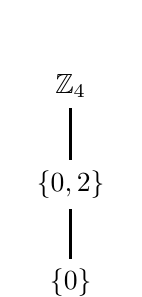
\begin{tikzpicture}[node distance=1.25cm,line width=1pt]
				\node(Z4) at (0,0)     {$\Zn{4}$};
				\node(02)       [below of =Z4] {$\{0,2\}$};
				\node(0)      [below of =02]  {$\{0\}$};
				\draw(Z4) -- (02);
				\draw(02) -- (0);
			\end{tikzpicture}
			\caption{$\Zn{4}$}
		\end{subfigure}%
		%\quad
		\begin{subfigure}[b]{0.25\textwidth}
			\centering
			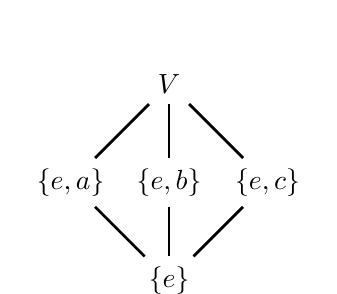
\begin{tikzpicture}[node distance=1.25cm,line width=1pt]
				\node(V) at (0,0)     {$V$};
				\node(eb)       [below of =V] {$\{e,b\}$};
				\node(ea)       [left of =eb] {$\{e,a\}$};
				\node(ec)       [right of =eb] {$\{e,c\}$};
				\node(e)      [below of =eb]  {$\{e\}$};
			 	\draw(V) -- (eb);
			 	\draw(eb) -- (e);
			 	\draw(V) -- (ea);
			 	\draw(V) -- (ec);
			 	\draw(ea) -- (e);
			 	\draw(ec) -- (e);
			\end{tikzpicture}
			\caption{$V$}
		\end{subfigure}
		\begin{subfigure}[b]{0.1\textwidth}
			\centering
			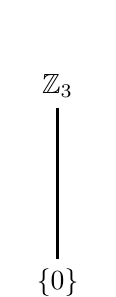
\begin{tikzpicture}[node distance=2.5cm,line width=1pt]
				\node(Z3) at (0,0)     {$\Zn{3}$};
				\node(0)      [below of =Z3]  {$\{0\}$};
			 	\draw(Z3) -- (0);
			\end{tikzpicture}
				\caption{$\Zn{3}$}
		\end{subfigure}
		\caption{Subgroup diagrams for $\Zn{4}$, $V$, and $\Zn{3}$}
	\end{figure}
\end{example}

\begin{definition}
	Let $H \leqslant G$. Then,
	\begin{enumerate}
		\item $H$ is the \textbf{trivial subgroup} if $H=\{e\}$.
		\item $H$ is a \textbf{non trivial subgroup} if $H \neq \{e\}$.
		\item $H$ is a \textbf{proper subgroup} if $H \neq G$.
		\item $H$ is the \textbf{improper subgroup} if $H = G$. \\
	\end{enumerate}
\end{definition}

\begin{theorem}
	Let $G$ be a group. $H \leqslant G$ is equivalent to, 
	\begin{enumerate}
		\item $H$ is closed under $\ast$.
		\item $e \in H$ where $e$ is the identity element of $G$.
		\item $\forall a \in H : \exists a^{-1} \in H$. \\
	\end{enumerate}
\end{theorem}

\begin{example}
	Consider $GL_2 (\mathbb{R})$ and $SL_2(\mathbb{R})$. Using \textbf{Thm 6}, we can show that $SL_2(\mathbb{R}) \leqslant GL_2(\mathbb{R})$.
	\begin{enumerate}
		\item $SL_2(\mathbb{R})$ is closed under matrix multiplication as for any $A,B \in SL_2(\mathbb{R})$,  $det(AB)=det(A)det(B)=1 \implies AB \in SL_2(\mathbb{R})$.
		\item The identity element $I_2$ is also in $SL_2(\mathbb{R})$ as $det(I_2)=1$.
		\item And for any $A \in SL_2(\mathbb{R})$, $A^{-1} \in SL_2(\mathbb{R})$ as $det(A^{-1})=det(A)^{-1}=1$.\\
	\end{enumerate}
\end{example}

\begin{theorem}
	Suppose $\phi : G \to G'$ is a group isomorphism with $H \leqslant G$. Then $\phi(H)=\{\phi(h) : h\in H \}$ is a subgroup in $G'$, i.e $\phi(H) \leqslant G'$.\\
\end{theorem}

\begin{proof}
\nextline
\begin{enumerate}
	\item As $\phi$ is a group isomorphism, for any $h_1' ,h_2' \in \phi(H) : h_1'h_2' = \phi(h_1h_2)\in \phi(H) $, which implies that it is closed.
	\item As $H \leqslant G$, $e \in H$. Thus $\phi(e) \in \phi(H)$ where $\phi(e)$ is the identity element of $G'$.
	\item For $\forall h'=\phi(h) \in \phi(H)$, there exists the inverse of it, $\phi(h^{-1})$ and the existence of such element is guranteed as $H\leqslant G$. 
\end{enumerate}
\end{proof}

\begin{definition}
	Let $G$ be a group where $a\in G$, we define $\cyc{a}=\{a^n : n \in \mathbb{Z} \}$\\
\end{definition}

\begin{theorem}
	Let $G$ be a group where $a\in G$. Then $\cyc{a}$ is the smallest subgroup of $G$ containing $a$.\\
\end{theorem}

\begin{proof}
\nextline 
\begin{enumerate}
	\item $\cyc{a}$ is closed under $\ast$ as for $a^i , a^j \in \cyc{a} \implies a^i \ast a^j = a^{i+j} \in \cyc{a}$.
	\item Identity element exists.
	\vskip 0.5ex
	$e\in \cyc{a}$ as $a^0 = e$.
	\item Inverse element exists.
	\vskip 0.5ex
	For $\forall a^i \in \cyc{a}$ there exists $(a^i)^{-1} = a^{-i}$ and as $i \in \mathbb{Z} \implies -i \in \mathbb{Z}$, thus the inverse of $\forall a^i \in \cyc{a}$,  $(a^i)^{-1} \in \cyc{a}$.
	\item It is the smallest subgroup containing $a$.
	\vskip 0.5ex
	It suffices to show that $a \in H' \leqslant G \implies \cyc{a} \subseteq H'$. Since $a \in H'$ and $H' \leqslant G$, $e=a^0 \in H'$ and $a^{-1} \in H'$. Since $H'$ is closed under $\ast$ and $a,a^{-1} \in H$, $a^n$ for $\forall n \in \mathbb{Z}$ are also elements of $H'$. This implies that $\cyc{a} \subseteq H$.
\end{enumerate}
\end{proof}

\begin{definition}
	Let $G$ be a group and $a \in G$.
	\begin{enumerate}
		\item $\cyc{a}$ is the \textbf{cyclic subgroup} of $G$, \textbf{generated} by $a$. The element $a$ is called the \textbf{generator} of $\cyc{a}$. 
		\item If $G=\cyc{a}$ for some $a \in G$, then $G$ is \textbf{cyclic}.\\
	\end{enumerate}
\end{definition}

\begin{example}
\nextline
\begin{enumerate}
	\item $\Zn{3}$ is cyclic since $\Zn{3}=\cyc{1}=\cyc{3}$.
	\item $V \simeq \Zn{2} \times \Zn{2}$ is not cyclic.
	\item $\mathbb{Q}$ is not cyclic.\\
\end{enumerate}
\end{example}

\vspace{0.25in}
\section{Cyclic Groups}
\vspace{0.25in}

\begin{definition}
	The \textbf{order of an element} $a\in G$ of a group $G$ is defined as $|\cyc{a}|$ which is also the smallest $n\in \mathbb{N}$ such that $a^n=e$ and denote it as $\mathcal{O}(a)$.\\
\end{definition}

\begin{remark}
	Do not get confused between order of groups and order of elements.\\
\end{remark}

\begin{theorem}
	If $G$ is a cyclic group which is generated by $a \in G$ then,
	\begin{equation}\nonumber
		G \simeq 
		\begin{cases}
		\Zn{n} & \mathcal{O}(a)\in\mathbb{N} \\ 
		\mathbb{Z} & \mathcal{O}(a) = \infty
		\end{cases}
	\end{equation}
\end{theorem}

\begin{proof}
\nextline
\begin{enumerate}
	\item $\mathcal{O}(a)\in\mathbb{N}$
	\vskip .5ex
	Let $\phi: G \to \Zn{n}$ which maps $\phi(a^i)=i$. Since $|G|=|\Zn{n}|=n$ such map is bijective. We can also show that it is a homomorphism. Thus such map suffices to be an isomorphism, which implies that $G \simeq \Zn{n}$.
	\item $\mathcal{O}(a)=\infty$
	\vskip .5ex
	Again let $\phi: G \to \mathbb{Z}$ by $\phi(a^i)=i$. Same as the above case we can show that $\phi$ is an isomorphism.
\end{enumerate}
\end{proof}

\begin{theorem}
	Let $G,G'$ be groups.
	\begin{enumerate}
		\item A cyclic group is abelian.
		\item If $\phi:G\to G'$ is an isomorphism and $G$ is cyclic then $G'$ is also cyclic.
		\item Suppose $\phi,\psi:G\to G'$ are both homomorphisms and $G=\cyc{a}$. If $\phi(a)=\psi(a)$, then $\phi=\psi$.\\
	\end{enumerate}
\end{theorem}

\begin{proof}
\nextline
\begin{enumerate}
	\item Let $G=\cyc{a}$. Then $a^i a^j = a^{i+j} = a^j a^i$ for every $i,j$, thus $G$ is abelian.
	\item Let $G=\cyc{a}$. We claim that $G'=\cyc{\phi(a)}$. It is obvious that $\cyc{\phi(a)}\subseteq G'$. Let $y\in G'$. Since $\phi$ is surjective, there exists some $a^i \in G$ such that $\phi(a^i)=y$. And since $\phi$ is a homomorphism, $y=\phi(a^i)=\phi(a\dots a)=\phi(a)^i \in \cyc{\phi(a)}$, which implies that $G'\subseteq\cyc{\phi(a)}$. Thus $G'=\cyc{\phi(a)}$.
	\item Let $G=\cyc{a}$. Then $\forall x \in G$, there exists some $i \in \mathbb{Z}$ such that $x=a^i$. Then $\phi(x)=\phi(a^i)=\phi(a\dots a)=\phi(a)^i$ as $\phi$ is an isomorphism. As we assumed that $\phi(a)=\psi(a)$, we can see that $\phi(x)=\phi(a)^i=\psi(a)^i=\psi(a^i)=\psi(x)$. As this holds for every $x \in G$, $\psi=\phi$.
\end{enumerate}
\end{proof}

\begin{remark}
	As any cyclic group is abelian, and any group generated by an element is cyclic, we can always get an abelian subgroup of any group even it is non abelian. For instance consider the non abelian group $GL_n(\mathbb{R})$ where $M\in GL_n(\mathbb{R})$. Then $\cyc{M}$ is abelian as it is cyclic, and it suffices $\cyc{M}\leqslant GL_n(\mathbb{R})$ due to \textbf{Thm 8}.\\
\end{remark}


\begin{remark}
	$V,\mathbb{Q},\mathbb{R}$ are abelian but not cyclic.\\
\end{remark}

\begin{theorem}
	Every subgroup of a cyclic group is cyclic.\\
\end{theorem}

\begin{proof}
	Suppose $G$ is a cyclic group and $H \leqslant G$. If $G$ is a trivial group, $H$ is also a trivial group which trivially suffices the theorem. Thus we will only consider cyclic groups with order greater than 1. Let it $G=\cyc{a}$ where $a\neq e$.
	\begin{enumerate}[label=(\roman*)]
		\item $H=\{e\}$ : cyclic
		\item $H\neq\{e\}$
		\vskip 0.5ex
		Let $n$ be the smallest positive integer such that $a^n \in H$. We claim that $H=\cyc{a^n}$. 
		\begin{enumerate}
			\item $\cyc{a^n} \subset H$
			\vskip 0.5ex
				It is obvious that $\cyc{a^n} \subset H$ since $a^n \in H$ and $H$ is closed under operation. 
			\item $H \subset \cyc{a^n}$
			\vskip 0.5ex
			Since $b \in G = \cyc{a}$ there exists some $m\in \mathbb{Z}$ such that $a^m=b$. Then $m=qn+r$ for some $q,r \in \mathbb{Z}$ such that $0 \leq r \leq n-1$. Then $b= a^m = a^{qn+r}=(a^q)^n a^r$, which again implies that $a^r=a^m (a^n)^{-q}$. As $a^m,(a^n)^{-q} \in H$, it implies that $a^r \in H$. Since $n$ was the smallest integer that makes $a^n\in H$ and $0\leq r \leq n-1$, $r$ should be 0. So as $m=qn+r=qn$, $b=a^m = a^qn = (a^n)^q$ for some $q \in \mathbb{Z}$. Thus for any $b \in H \implies b \in \cyc{a^n}$. 
		\end{enumerate}
	Thus due to a) and b) we conclude that $H=\cyc{a^n}$ which is a cyclic group.
	\end{enumerate}
\end{proof}

\begin{remark}
	If $n|m$ for $n,m\in\mathbb{Z} \implies \cyc{a^m}\subset \cyc{a^n}$.\\
\end{remark}

Now we know that for any cyclic groups, their subgroups are also cyclic. We also know that if some group is cyclic, it is isomorphic to $\mathbb{Z}$ or $\Zn{n}$ for some $n$ which is the order of the generator of the group. This implies that cyclic groups are all about $\Zn{n}$, and its subgroups. The next theorem states about subgroups of $\Zn{n}$ and which ones are identical. For example consider $\cyc{28} \in \Zn{108}$, we can just derive the group by keep adding up 28 and get the $mod$ 108 value. Using the next theorem, we can easily consider certain subgroups of $\Zn{n}$ by considering the divisibility between the order of the element and the order of the group.\\

\begin{theorem}
	Let $G=\cyc{a}$ and $\mathcal{O}(a)=n$.\\
	\begin{enumerate}
		\item $\mathcal{O}(a^s)=\frac{n}{gcd(n,s)}$ for $s\in\mathbb{Z}$.
		\item For each $m$ such that $m|n$ there exists exactly one subgroup of order $m$, which is $\cyc{a^{n/m}}$.
		\item $\cyc{a^s}=\cyc{a^t} \iff gcd(n,s)=gcd(n,t)$.\\
	\end{enumerate}
\end{theorem}

\begin{proof}
\nextline
\begin{enumerate}
	\item $\mathcal{O}(a^s)=\frac{n}{gcd(n,s)}$ for $s\in\mathbb{Z}$
	\vskip 0.5ex
	Let $m=\mathcal{O}(a^s)$ which implies $(a^s)^m = a^{sm} =e$ in $G=\cyc{a}$. As $\mathcal{O}(a)=n$, it follows that $n \mid sm$. Then, \\
	\begin{equation}\nonumber
		\begin{split}
		n | sm &\implies \frac{n}{gcd(n,s)} \mid \frac{s}{gcd(n,s)} m\\
		&\implies \frac{n}{gcd(n,s)} \mid m \\
		\end{split}
	\end{equation}\\
	where the second implication was derived by the fact that $ \frac{n}{gcd(n,s)}\nmid \frac{s}{gcd(n,s)}$. So as $m$ is the smallest integer that should satisfy the above relation, $m=\mathcal{O}(a^s)=\frac{n}{gcd(n,s)}$.
	\item  There exists exactly one subgroup of order $m : m |n$, which is $\cyc{a^{n/m}}$.
	\vskip 0.5ex
%	First we will show that $\cyc{a^\frac{n}{m}}$ suffices the statement. 
	Suppose $H \leqslant G$ and $|H|=m$. Also as $H$ is a subgroup of a cyclic group it is also cyclic, which implies that $H=\cyc{a^s}$ for some $s\in\mathbb{Z}$. Then due to 1,\\
	\begin{equation}\nonumber
		|H| =\mathcal{O}(a^s) = \frac{n}{gcd(n,s)} = m
	\end{equation}\\
	which implies that $gcd(n,s)=\frac{n}{m} \implies \frac{n}{m} \mid s$. Recall that $\frac{n}{m} \mid s \implies \cyc{a^s} \subset \cyc{a^\frac{n}{m}}$. But as $\mathcal{O}(a^s)=\mathcal{O}(a^\frac{n}{m})=m$, it should satisfy that $\cyc{a^\frac{n}{m}}=\cyc{a^s}$.
	\item  $\cyc{a^s}=\cyc{a^t} \iff gcd(n,s)=gcd(n,t)$.
	\vskip 0.5ex
	\begin{enumerate}[label=(\roman*)]
		\item $\cyc{a^s}=\cyc{a^t} \implies gcd(n,s)=gcd(n,t)$.
	%	\vskip 0.5ex
		\begin{equation}\nonumber
			\begin{split}
			\cyc{a^s}=\cyc{a^t} &\implies |\cyc{a^s}|=|\cyc{a^t}| \\
			&\iff \frac{n}{gcd(n,s)} = \frac{n}{gcd(n,t)} \\
			&\iff gcd(n,s) = gcd(n,t)
			\end{split}
		\end{equation} \\
		\item $\cyc{a^s}=\cyc{a^t} \impliedby gcd(n,s)=gcd(n,t)$
		\vskip 0.5ex
		Using the result of 2, we can show that $\cyc{a^s}=\cyc{a^t} \impliedby |\cyc{a^s}|=|\cyc{a^t}| $ and using the implications used in (i), we derive that $\cyc{a^s}=\cyc{a^t} \impliedby gcd(n,s)=gcd(n,t)$.
	\end{enumerate}
\end{enumerate}
\end{proof}

We abused the notation of $gcd(n,m)$ without defining it, and even assuming that we all know it. We define the greatest common divisor using group theoretic notions. \\

\begin{definition}
	The \textbf{greatest common divisor} of $r,s \in \mathbb{Z}$, is an integer $d\in \mathbb{Z}$ which suffices $\cyc{d} = \{nr+ms : n,m\in \mathbb{Z} \}$, and denote it as $d=gcd(r,s)$. We say that $r$ and $s$ are \textbf{coprime}, or \textbf{relatively prime} if $gcd(r,s)=1$.\\
\end{definition}

\begin{theorem}
	Let $r,s \in \mathbb{Z}$.
	\begin{enumerate}
		\item $gcd(r,s) \mid r$ and $gcd(r,s) \mid s$.
		\item If $d' \mid r$ and $d' \mid s$, then $d' \mid gcd(r,s)$.
		\item $gcd(r,s)=1$ and $r\mid sm \implies r \mid m$.\\
	\end{enumerate}
\end{theorem}

\begin{proof}
\nextline
\begin{enumerate}
	\item As $\cyc{gcd(r,s)}=\{nr+ms : n,m\in \mathbb{Z} \} , \implies gcd(r,s) \mid nr+ms$. Let $n=0 , m=1$ then $gcd(r,s) \mid nr+ms \implies gcd(r,s) \mid s$. Also if we let $n=1, m=0$ then $gcd(r,s) \mid nr+ms \implies gcd(r,s) \mid r$.
	\item $gcd(r,s)=nr+ms$ for some $n,m \in \mathbb{Z}$. As $d' \mid r$ and $d' \mid s$, for such $n,m$, $d' \mid nr+ms =d$. Thus $d' \mid d$.
	\item Since $gcd(r,s)=1 \implies \exists n_0 , m_0 \in \mathbb{Z}: n_0 r + m_0 s = gcd(r,s)=1$. Then $mn_0 r + mm_0 s =m$. Since $r \mid n_0 m r$ and $r \mid sm \implies r\mid m_0 sm$, we can see that $r \mid mn_0 r + mm_0 s = m$. Thus $r \mid m$.
\end{enumerate}
\end{proof}

\begin{remark}
	Since  $\cyc{gcd(r,s)}=\{nr+ms : n,m\in \mathbb{Z} \} $ the problem of finding the greatest common divisor can be viewed in a different perspective, of finding two integers. This can sometimes ease the computational complexity of using prime factorization for calculating greatest common divisors, as finding prime itself is also a quite not so easy problem.
\end{remark}
\end{document}